\chapter{Motivation for Higgs Sector Extensions and Higgs CP Studies}
\chaptermark{Motivation for Higgs Sector Extensions and Higgs CP Studies}  
\thispagestyle{plain}  % First page has default style
\pagestyle{chapterpages}
\label{Section:Chapter2}

In Chapter~\ref{Section:Chapter1}, the SM of particle physics was explored to establish the theoretical foundation of this work. While the SM has been immensely successful, with its predictions verified experimentally to a high degree of precision, it remains an incomplete theory of nature due to several fundamental theoretical problems. Beyond these theoretical issues, the emergence of experimental results in tension with SM predictions has sparked significant interest among particle physicists. Although the statistical significance of these tensions is not yet sufficient to claim new discoveries, the search for BSM physics to explain them remains an intriguing and active area of research. This chapter will focus on two major theoretical challenges; the hierarchy problem and the observed matter-antimatter asymmetry of the universe, while also briefly discussing key experimental tensions. Possible solutions within the context of BSM physics will then be explored, with the observed Higgs boson playing an integral role in the matter-antimatter asymmetry discussion.

\section{Hierarchy problem}
With these fundamental problems in mind, it seems fairly clear that the SM is an \ac{EFT}, describing physics up to a certain energy scale. However, an extension is required to describe physics at the Planck scale ($10^{19}\GeV$) where gravitational effects become significant. The hierarchy problem is a central issue in the Higgs sector arising from the absence of a natural mechanism to stabilise the Higgs mass against large quantum corrections.

In QFT, the Higgs boson mass in not simply a fixed parameter, receiving corrections to its physical mass from virtual processes involving particles that couple directly or indirectly to the Higgs field. Mathematically the physical mass of the Higgs boson can be expressed as

\begin{equation}
    m_H^2 = (m_H^0)^2 + \Delta m_H^2
\label{Equation:Chapter2_HiggsBosonMass}
\end{equation}

where $m_H^0$ represent the bare mass of the Higgs boson, and $\Delta m_H$ term encapsulates the quantum loop corrections from these virtual particle interactions with this loop-induced correction taking the following form in the EFT framework

\begin{equation}
    \Delta m_H^2 = -\frac{g_f^2}{8\pi^2}\Lambda^2 + \space \text{...}
\end{equation}

where $\Lambda$ should be interpreted as the least energy scale at which new physics is expected to modify the high-energy behaviour of the theory. The Feynman diagram for the mass correction due to a fermion coupling to the Higgs field is shown in Fig.~\ref{Figure:Chapter2_Hierarchy_Feynman1}.

\begin{figure}[h]
\centering
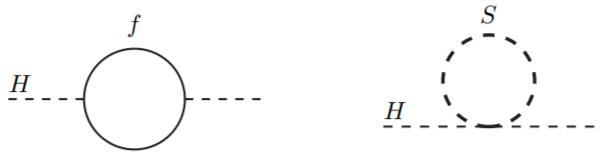
\includegraphics[width= 0.9\textwidth]{Figures/Chapter2/Hierarchy_Feynman_1.png}
\caption{TODO}
\label{Figure:Chapter2_Hierarchy_Feynman1}
\end{figure}

At the core of the hierarchy problem lies this $\Lambda$ term as the current best measurement of the Higgs boson mass from the Compact Muon Solenoid at $125.38 \pm 0.14~\GeV$ (in natural units), can only be explained if there is an extreme degree of fine-tuning in Eq.~\ref{Equation:Chapter2_HiggsBosonMass}. Specifically, if $\Lambda$ is taken to be the Plank scale, the predicted Higgs boson mass would be many orders of magnitude larger than the observed value ($\propto \Lambda^2$). Reconciling this discrepancy requires that the bare mass term is sufficiently large ($\mathcal{O}(10^{38})$ to cancel out the quantum loop correction term.

Perhaps, the most studied and appealing solution to the hierarchy problem is \ac{SUSY}, which introduces a symmetry relating fermions and bosons. In SUSY, every known SM particle has at least one supersymmetric partner: bosons have fermionic superpartners while, fermions have scalar boson superpartners. This symmetry provides a natural way of addressing this extreme fine-tuning, as superpartners also contribute to $\Delta m_H^2$ but, with opposite signs relative to their SM counterparts, allowing the Higgs mass to stabilise naturally through the cancellation of the quantum loop corrections. The Feynman diagram for the mass correction due to a fermionic superpartner (scalar boson) is shown in Fig.~\ref{Figure:Chapter2_Hierarchy_Feynman2}.

\begin{figure}[h]
\centering
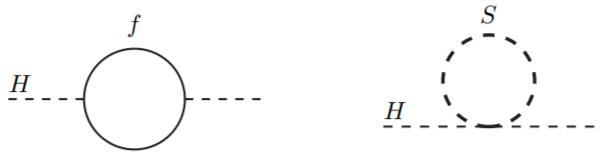
\includegraphics[width= 0.9\textwidth]{Figures/Chapter2/Hierarchy_Feynman_1.png}
\caption{TODO}
\label{Figure:Chapter2_Hierarchy_Feynman2}
\end{figure}

While SUSY provides a natural solution to the hierarchy problem, the lack of any experimental evidence for supersymmetric partners, along with strong experimental constraints on the simplest SUSY extension of the SM (MSSM), has lead to alternative extensions to the SM Higgs sector gaining traction. One such extension is the \ac{2HDM}, which could provide a way to mitigate the fine-tuning in the Higgs mass by introducing additional Higgs bosons that could alter the running of coupling constants and loop corrections. Moreover, 2HDMs are particularly interesting in light of the muon $g-2$ anomaly, which will be discussed in this chapter.

\section{Extended Higgs sector - 2HDM}

The simplest extension to the SM Higgs sector is the 2HDM which comprises of two complex scalar $SU(2)_L$ doublets, $\Phi_1$ and $\Phi_2$

\begin{equation}
\Phi_i =
\begin{pmatrix}
\phi_i^{+} \\
\phi_i^{0} 
\end{pmatrix}
\quad ,\quad i = 1,2
\end{equation}

To preserve the $U(1)_{EM}$ symmetry, only the neutral components of the Higgs doublets acquire non-zero VEVs

\begin{equation}
    <0|\Phi_i|0> = \frac{1}{\sqrt{2}} \begin{pmatrix}
        0 \\
        \nu_i
    \end{pmatrix} \quad,\quad i=1,2
\end{equation}

where $\nu_i$ represents the VEVs of each Higgs doublet.

In contrast to the SM Higgs potential, the 2HDM counterpart exhibits an extended form because of the presence of the additional doublet

\begin{equation}
\begin{array}{c}
    V(\phi_1,\phi_2) = m_{11}^2 \phi_1^{\dagger}\phi_1 + m_{22}^2 \phi_2^{\dagger}\phi_2 - m_{12}^2(\phi_1^\dagger\phi_2 + \text{H.c.}) \\
    + \frac{1}{2} \lambda_1(\phi_1^\dagger\phi_1)^2 + \frac{1}{2}\lambda_2(\phi_2^\dagger\phi_2)^2 + \lambda_3(\phi_1^\dagger\phi_1)(\phi_2^\dagger\phi_2) \\
    + \lambda_4(\phi_1^\dagger\phi_2)(\phi_2^\dagger\phi_1) + \frac{1}{2}\lambda_5[(\phi_1^\dagger\phi_2)^2 + \text{H.c.}] \\
\end{array}
\end{equation}

where the doublet scalar potential is expressed in terms of the mass parameters ($m_{ij}$) and the quartic couplings ($\lambda_i$).

After SSB, the Higgs doublets can be expanded around the minima

\begin{equation}
    \Phi_i = \begin{pmatrix}
        \phi_i^+ \\
        \frac{1}{\sqrt{2}}(\nu_i + h_i + iz_i
    \end{pmatrix} \quad,\quad i=1,2
\end{equation}

where the doublets have been expressed in terms of CP-even ($h_i$), CP-odd ($z_i$) and charged Higgs fields ($\phi_i^+$).

Analogous to the SM Higgs sector, the inclusion of a second Higgs doublet introduces an additional 4 dof. Upon SSB, 3 out of the 8 dof are absorbed as Goldstone bosons providing the W$^{\pm}$ and Z bosons with longitudinal dof while the remaining 5 dof correspond to 5 physical Higgs bosons; 2 CP-even (h and H), 1 CP-odd (A) and 2 charged Higgs bosons (H$^{\pm}$). The mass eigenstates corresponding to these physical Higgs bosons are admixtures of the components of the two Higgs doublets in Eq.~\ref{Equation:Chapter2_2HDM-MassEigenstates}.

\begin{equation}
\begin{array}{c}
     h = h_1 \sin{\alpha} - h_2 \cos{\alpha} \\
     H = - h_1 \cos{\alpha} - h_2 \sin{\alpha} \\
     H^\pm = \phi_1^+ \sin{\beta} + \phi_2^+ \cos{\beta} \\
     A = z_1 \sin{\beta} - z_2 \cos{\beta}
\end{array}
\label{Equation:Chapter2_2HDM-MassEigenstates}
\end{equation}

where the parameter $\alpha$ governs the mixing between the CP-even scalars and $\beta$ is a rotational angle that diagonalises the mass-squared matrices of the pseudoscalar and the charged Higgs, defined as $\tan{\beta} = \nu_2/\nu_1$.

A major constraint imposed to 2HDMs is suppressing tree-level flavour-changing neutral currents which can occur in a generic 2HDM because of both Higgs doublet coupling to the same fermion flavour, leading to non-diagonal Yukawa couplings after SSB. To forbid these tree-level interactions, a discrete $\mathbb{Z}_2$ symmetry \cite{2HDM(2)} is introduced, $\Phi_1 \to \Phi_1$, $\Phi_2 \to - \Phi_2$, $\Phi_1 \not\to \Phi_2$, which eliminates the $\lambda_6$ and $\lambda_7$ terms from the scalar potential in Eq.~\ref{Equation:Chapter2_2HDMScalarPotential}. Rather than being strictly imposed, this $\mathbb{Z}_2$ symmetry is softly broken by the $m_{12}^2$ term in the scalar potential. This soft-breaking of the symmetry allows the Yukawa couplings to remain flavour diagonal while, simultaneously allowing for mixing between the Higgs doublets ($\Phi_i$), which is required to obtain the physical Higgs mass eigenstates. Following the introduction of $\mathbb{Z}_2$ symmetry, the CP-conserving 2HDMs are split in different types, which are defined based on which Higgs doublet couples to each fermion flavour. The four types of CP-conserving 2HDMs are shown in Table~\ref{Table:Chapter2_2HDM-Types}.

\begin{table}[h]
\centering
\renewcommand{\arraystretch}{1.5} % Increase row height
\setlength{\tabcolsep}{12pt} % Increase column width
\arrayrulecolor{black} % Ensure outer borders are black
\begin{tabular}{|c|c|c|c|c|}
\hline
    & Type I   & Type II  & Type X   & Type Y   \\ \hline \hline
$u$ & $\Phi_2$ & $\Phi_2$ & $\Phi_2$ & $\Phi_2$ \\ 
\arrayrulecolor{lightgray} \hline
$d$ & $\Phi_2$ & $\Phi_1$ & $\Phi_2$ & $\Phi_1$ \\ 
\arrayrulecolor{lightgray} \hline
$l$ & $\Phi_2$ & $\Phi_2$ & $\Phi_1$ & $\Phi_2$ \\ 
\arrayrulecolor{black} \hline
\end{tabular}
\caption{TODO}
\label{Table:Chapter2_2HDM-Types}
\end{table}

In each 2HDM type, the structure of the Yukawa interactions depend on the specific assignment of the fermion couplings to the Higgs doublets. After SSB, the Yukawa part of the 2HDM Lagrangian can be expressed in terms of the physical Higgs mass eigenstates, up-like ($u$) and down-like($d$) quark, charged lepton ($l$) and neutrino ($\upsilon$) fields as

\begin{equation}
\begin{aligned}
    \mathcal{L}_{Yukawa}^{2HDM} &= - \sum\limits_{f=u,d,l} \frac{m_f}{\nu} 
    \left(g_f^h \overline{f}f h + g_f^H\overline{f}f H - i g_f^A\overline{f} \gamma_5 f A \right) \\
    &\quad - \left\{ \frac{\sqrt{2}V_{ud}}{\nu} \overline{u} 
    \left(m_u g_u^A P_L + m_d g_d^A P_R \right) d H^+ \right. \\
    &\quad \left. + \frac{\sqrt{2}m_l g_{l}^A}{\nu} \overline{\upsilon
_L} l_R H^+ + H.c. \right\}
\end{aligned}
\label{Equation:Chapter2_2HDM-YukawaLagrangian}
\end{equation}

where $g_f^H,g_f^A,g_f^h$ are the normalised Yukawa couplings of the fermions to the Higgs mass eigenstates, expressed relative to the SM Higgs boson's couplings. These couplings are summarised in Table~\ref{Table:Chapter2_2HDM-Couplings} for each of the four types of 2HDMs.


\begin{table}[h]
\centering
\renewcommand{\arraystretch}{1.5} % Increase row height
\setlength{\tabcolsep}{12pt} % Increase column width
\arrayrulecolor{black} % Ensure outer borders are black
\begin{tabular}{|c|c|c|c|c|}
\hline
        & Type I                     & Type II                     & Type X                                        & Type Y                      \\ \hline \hline
$g_l^A$ & $1/\tan{\beta}$            & $\tan{\beta}$               & $\tan{\beta}$    & $-1/\tan{\beta}$            \\ \arrayrulecolor{lightgray} \hline
$g_u^A$ & $1/\tan{\beta}$            & $1/\tan{\beta}$             & $1/\tan{\beta}$                               & $1/\tan{\beta}$             \\ \arrayrulecolor{lightgray} \hline
$g_d^A$ & $1/\tan{\beta}$            & $\tan{\beta}$               & $-1/\tan{\beta}$                              & $\tan{\beta}$               \\ \arrayrulecolor{lightgray} \hline
$g_l^H$ & $\sin{\alpha}/\sin{\beta}$ & $\cos{\alpha}/\cos{\beta}$  & $\cos{\alpha}/\cos{\beta}$                    & $\sin{\alpha}/\sin{\beta}$  \\ \arrayrulecolor{lightgray} \hline
$g_u^H$ & $\sin{\alpha}/\sin{\beta}$ & $\sin{\alpha}/\sin{\beta}$  & $\sin{\alpha}/\sin{\beta}$                    & $\sin{\alpha}/\sin{\beta}$  \\ \arrayrulecolor{lightgray} \hline
$g_d^H$ & $\sin{\alpha}/\sin{\beta}$ & $\cos{\alpha}/\cos{\beta}$  & $\sin{\alpha}/\sin{\beta}$                    & $\cos{\alpha}/\cos{\beta}$  \\ \arrayrulecolor{lightgray} \hline
$g_l^h$ & $\cos{\alpha}/\sin{\beta}$ & $-\sin{\alpha}/\cos{\beta}$ & $-\sin{\alpha}/\cos{\beta}$                   & $\cos{\alpha}/\sin{\beta}$  \\ \arrayrulecolor{lightgray} \hline
$g_u^h$ & $\cos{\alpha}/\sin{\beta}$ & $\cos{\alpha}/\sin{\beta}$  & $\cos{\alpha}/\sin{\beta}$                    & $\cos{\alpha}/\sin{\beta}$  \\ \arrayrulecolor{lightgray} \hline
$g_d^h$ & $\cos{\alpha}/\sin{\beta}$ & $-\sin{\alpha}/\cos{\beta}$ & $\cos{\alpha}/\sin{\beta}$                    & $-\sin{\alpha}/\cos{\beta}$ \\ \arrayrulecolor{black} \hline
\end{tabular}
\caption{TODO}
\label{Table:Chapter2_2HDM-Couplings}
\end{table}

In 2HDMs, the observed Higgs boson can be matched to the predicted CP-even bosons by a linear combination of the two mass eigenstates 

\begin{equation}
    h_{\text{obs}} = \sin{(\beta - \alpha)} h + \cos{(\beta - \alpha)} H 
\end{equation}

In the Higgs alignment limit, one of these CP-even neutral Higgs boson is the observed Higgs, which enables two possible alignment scenarios, the normal and inverted scenarios. In the normal scenario, the observed Higgs is identified as the lighter h in 2HDM, in contrast to H being identified as the observed Higgs in the inverted scenario (Eqs.~\ref{Equation:Chapter2-NormalScenario,Equation:Chapter2-InvertedScenario}. The adjusted couplings of the unmatched CP-even boson are summarised in Table~\ref{Table:Chapter2_2HDM-CouplingsAlignmentLimit} for each of the four different types of 2HDMs.

\begin{equation}
\begin{rcases}
  h_{\text{obs}} = h \\
  \cos(\beta-\alpha) = 0 
\quad \end{rcases}
\quad \text{Normal}
\label{Equation:Chapter2-NormalScenario}
\end{equation}

\begin{equation}
\begin{rcases}
  h_{\text{obs}} = H \\
  \sin(\beta-\alpha) = 0
\quad \end{rcases}
\quad \text{Inverted}
\label{Equation:Chapter2-InvertedScenario}
\end{equation}


\begin{table}[h]
\centering
\renewcommand{\arraystretch}{1.5} % Increase row height
\setlength{\tabcolsep}{12pt} % Increase column width
\arrayrulecolor{black} % Ensure outer borders are black
\begin{tabular}{|c|c|c|c|c|}
\hline
Normal (Inverted)     & Type I                     & Type II                     & Type X                                        & Type Y                      \\ \hline \hline
(-)$g_l^{H(h)}$ & $-1/\tan{\beta}$  & $\tan{\beta}$  & $\tan{\beta}$                    & $-1/\tan{\beta}$  \\ \arrayrulecolor{lightgray} \hline
(-)$g_u^{H(h)}$ & $-1/\tan{\beta}$  & $-1/\tan{\beta}$  & $-1/\tan{\beta}$                    & $-1/\tan{\beta}$  \\ \arrayrulecolor{lightgray} \hline
(-)$g_d^{H(h)}$ & $-1/\tan{\beta}$  & $\tan{\beta}$  & $-1/\tan{\beta}$                    & $\tan{\beta}$  \\ \arrayrulecolor{black} \hline
\end{tabular}
\caption{TODO}
\label{Table:Chapter2_2HDM-CouplingsAlignmentLimit}
\end{table}

\section{\texorpdfstring{Muon $g$-2 anomaly}{Muon g-2 anomaly}}

In 2023, Fermilab announced the most precise measurement of the anomalous magnetic moment of the muon, $\alpha_\mu$. Combined with the earlier result from the Brookhaven National Laboratory, the experimental average of the muon anomaly exhibits a 5.0~$\sigma$ discrepancy from SM prediction compiled by the Muon $g-2$ Theory Initiative in 2020. This is a definitely an intriguing result, as it could be a hint of BSM physics, however, caution is also warranted, as there also tensions between the different theoretical calculations that could bring the prediction closer to the experimental value.


\begin{equation}
\begin{aligned}
    \alpha_\mu (SM) &= 116591810(43) \times 10^{-11} \\
    \alpha_\mu (\text{exp}) &= 116592059(22) \times 10^{-11} \quad (0.19~\text{ppm}) \\
    \Delta \alpha_\mu &= (249\pm48) \times 10^{-11}
\end{aligned}
\end{equation}

A possible explanation for the discrepancy between the experimental measurements and the theoretical prediction of the $g-2$ anomaly can be accommodated by 2HDMs. In 2HDMs, the additional Higgs bosons can introduce loop corrections to the calculation of $\alpha_\mu$, through one-loop and two-loop Barr-Zee interactions presented in Fig.~\ref{TODO} and Fig.~\ref{TODO} respectively. The one-loop contributions are mediated by $\phi$, A and H$^{\pm}$ with the contribution of $\phi$ to $\Delta\alpha_\mu$ being positive $\alpha_\mu$ while those of A and H$^{\pm}$ are negative. The dominant contribution comes from two-loop Barr-Zee type diagrams with heavy fermions in the loop providing a positive shift to $\Delta\alpha_\mu$, with the CP-odd Higgs boson contributing positively primarily through the top quark loop. However, the contribution from the additional CP-even boson can have either a positive or a negative impact, depending on $\tan{\beta}$. 



\section{The matter-antimatter asymmetry problem}
- The matter-antimatter asymmetry problem and why the SM fails to explain it
- The role of CP violation in baryogenesis
\section{CP Nature of the SM Higgs boson}
- CP Nature of Higgs:
- Why the observed Higgs may not be purely CP-even
- Connection between CP violation in the Higgs sector and new physics
- Higgs $\rightarrow \tau \tau$ as a Probe for CP Violation:
- Theoretical motivation for using tau leptons
- Experimental approaches to measuring CP violation in Higgs decays